% !TeX spellcheck = fr_FR
\chapter{Chapitre 10: Système d'authentification sécurisé}\label{chap:auth}

\section{Objectifs}
Nous avons conçu et mis en œuvre un système d'authentification complet, aligné sur les bonnes pratiques actuelles.

\section{Aperçu de l'architecture}
L'application utilise un schéma d'authentification dédié lié à une base de données MySQL distincte (\texttt{auth\_db}). Comme on l'a vu, les données principales de l'application demeurent dans \texttt{stops\_db}. Cette séparation réduit le rayon d'impact et garantit, entre autres, que la réimportation des données de transport public ne touche jamais aux identifiants des utilisateurs.

\subsection{Composants}
\begin{itemize}
  \item \textbf{Stockage des mots de passe} : Argon2id (argon2-cffi)\citeref{ref:argon2_docs}, à forte consommation mémoire, salé, avec des paramètres spécifiques à chaque hachage.
  \item \textbf{Sessions} : Flask-Login avec cookies sécurisés (HttpOnly, SameSite=Lax ; indicateur Secure en production).
  \item \textbf{CSRF} : Protection CSRF de Flask-WTF pour tous les formulaires POST et les points de terminaison concernés.
  \item \textbf{Limitation de débit} : Les routes de connexion et d'inscription sont limitées (Flask-Limiter) afin d'atténuer la force brute.
  \item \textbf{Sécurité du transport} : Flask-Talisman fournit les en-têtes de sécurité ; application stricte de HTTPS.
  \item \textbf{2FA} : TOTP (compatible Google Authenticator)\citeref{ref:totp_rfc} avec activation par QR code et codes de secours à usage unique. \textbf{Le secret TOTP est chiffré au repos} (Fernet)\citeref{ref:fernet_docs} ; les codes de secours sont hachés (Argon2).
  \item \textbf{Verrouillage de compte} : Verrouillage progressif après des échecs répétés, avec temporisation exponentielle.
  \item \textbf{Vérification d'email} : Liens signés (validité 48 h) envoyés à l'inscription et lors d'une connexion non vérifiée. La vérification est \emph{optionnelle par défaut}.
  \item \textbf{CAPTCHA} : Cloudflare Turnstile\citeref{ref:cloudflare_turnstile} sur \texttt{/auth/register} et \texttt{/auth/login}.
  \item \textbf{Journalisation d'audit} : enregistrement des événements d'authentification dans \texttt{auth\_db.auth\_events} et émission simultanée de logs JSON sur \texttt{stdout}
\end{itemize}

\section{Modèle de données (auth\_db)}
La table \texttt{users} stocke les comptes utilisateurs avec les champs suivants :

\begin{table}[H]
\centering
\caption{Champs de la table \texttt{users}}
\label{tab:chap10_users_fields}
\noindent\begin{tabular}{@{}p{0.40\linewidth}p{0.60\linewidth}@{}}
\textbf{Identité} & \texttt{email} (unique) \\
\hline
\textbf{Authentification} & \texttt{password\_hash} (Argon2id) \\
\hline
\textbf{Rôles} & \texttt{is\_admin} \\
\hline
\textbf{Vérification d'email} & \texttt{is\_email\_verified}, \texttt{email\_verified\_at}, \texttt{last\_verification\_sent\_at} \\
\hline
\textbf{2FA} & \texttt{is\_totp\_enabled}, \texttt{totp\_secret} \\
\hline
\textbf{Codes de secours} & JSON de hachés Argon2 \\
\hline
\textbf{Hygiène de compte} & \texttt{created\_at}, \texttt{updated\_at}, \texttt{last\_login\_at} \\
\hline
\textbf{Verrouillage} & \texttt{failed\_login\_attempts}, \texttt{locked\_until} \\
\end{tabular}
\end{table}


\subsection*{Journalisation d'audit (\texttt{auth\_events})}
\noindent Une table \texttt{auth\_events} (même schéma \texttt{auth\_db}) consigne les événements de sécurité :

\begin{table}[H]
\centering
\caption{Champs de la table \texttt{auth\_events}}
\label{tab:chap10_auth_events_fields}
\noindent\begin{tabular}{@{}p{0.40\linewidth}p{0.60\linewidth}@{}}
\textbf{Type d'événement} & \texttt{event\_type} (\textit{registration}, \textit{login\_success}, \textit{login\_failure}, \textit{account\_locked}, \textit{2fa\_success}, \textit{2fa\_failure}, \textit{2fa\_enabled}, \textit{2fa\_disabled}, \textit{email\_verified}) \\
\hline
\textbf{Utilisateur} & \texttt{user\_id} (nullable), \texttt{email\_attempted} (pour les échecs) \\
\hline
\textbf{Contexte} & \texttt{ip\_address}, \texttt{user\_agent} \\
\hline
\textbf{Détails} & \texttt{metadata\_json} \\
\hline
\textbf{Horodatage} & \texttt{occurred\_at} (UTC) \\
\end{tabular}
\end{table}

\begin{codebox}[language=Python]{Modèle minimal (extrait)}
class AuthEvent(db.Model):
    __bind_key__ = 'auth'
    __tablename__ = 'auth_events'
    id = db.Column(db.Integer, primary_key=True)
    user_id = db.Column(db.Integer, db.ForeignKey('users.id'), index=True)
    email_attempted = db.Column(db.String(255), index=True)
    event_type = db.Column(db.String(50), nullable=False, index=True)
    ip_address = db.Column(db.String(45))
    user_agent = db.Column(db.Text)
    metadata_json = db.Column(db.Text)
    occurred_at = db.Column(db.DateTime, default=utcnow, index=True)
\end{codebox}

\noindent Les mêmes événements sont émis au format JSON sur la sortie standard du service pour une collecte centralisée.
\subsection{Parcours utilisateur et impact sur les données}
Cette sous-section illustre, étape par étape, comment les actions de l'utilisateur se traduisent dans le schéma \texttt{auth\_db}.

\paragraph{Accès aux écrans d'authentification}
\begin{figure}[H]
  \centering
  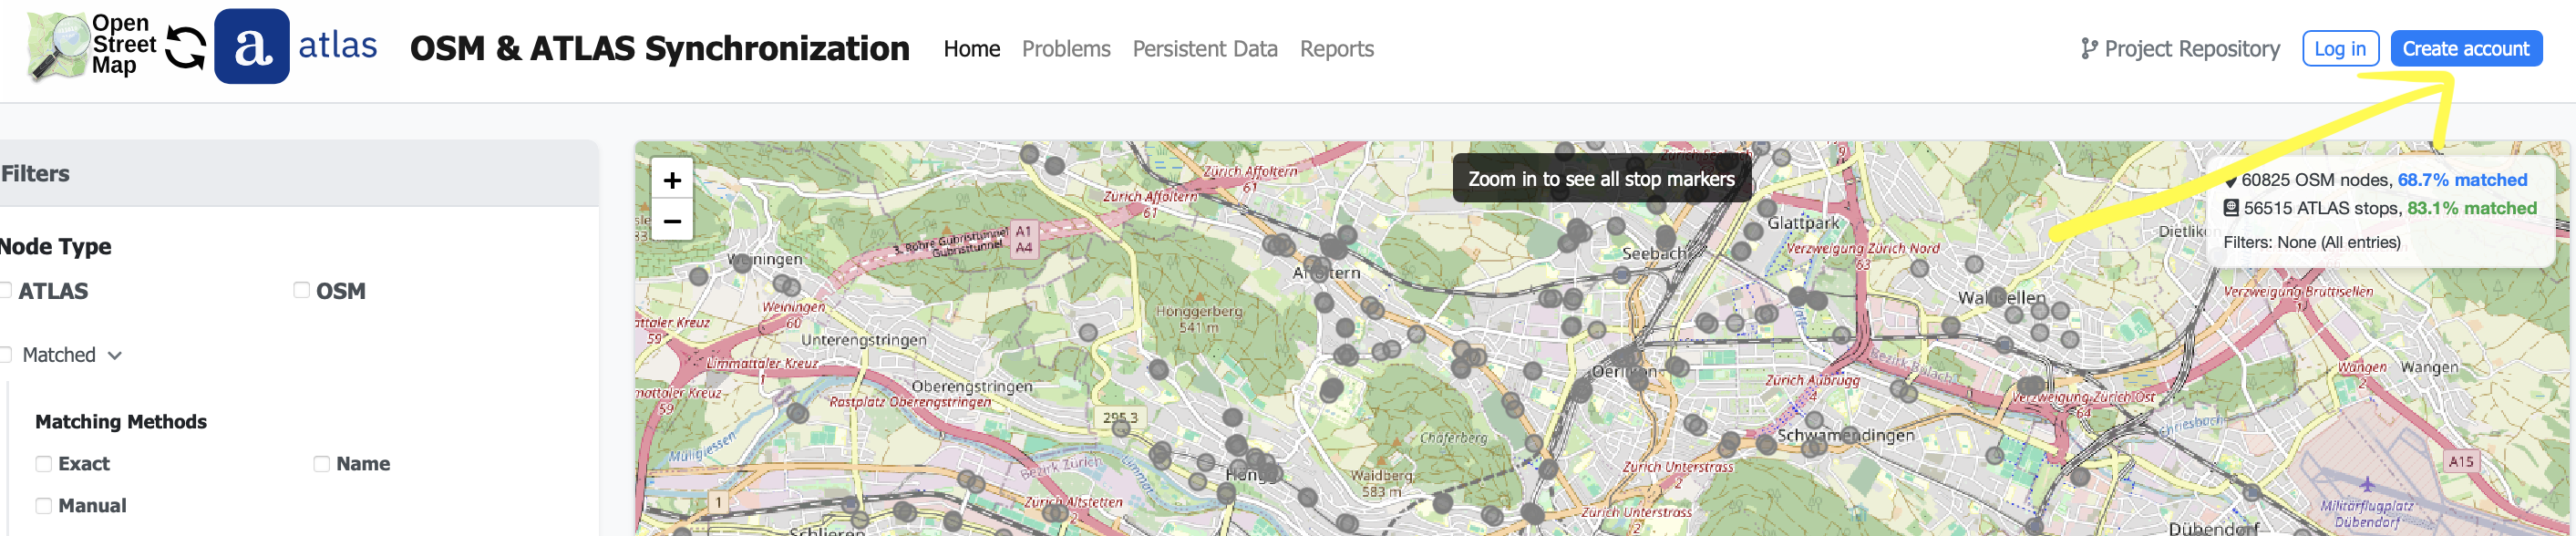
\includegraphics[width=0.85\textwidth]{../figures/chap10/auth1.png}
  \caption{Bouton \og Créer un compte \fg{} visible dans l'interface.}
\end{figure}

\paragraph{Inscription}
Un utilisateur fournit un email et un mot de passe ; le serveur hache le mot de passe avec Argon2id et crée la ligne dans \texttt{users}.

\begin{codebox}[language=Python]{Hachage du mot de passe (inscription)}
from argon2 import PasswordHasher
ph = PasswordHasher()
password_hash = ph.hash(plain_password)
\end{codebox}

\begin{figure}[H]
  \centering
  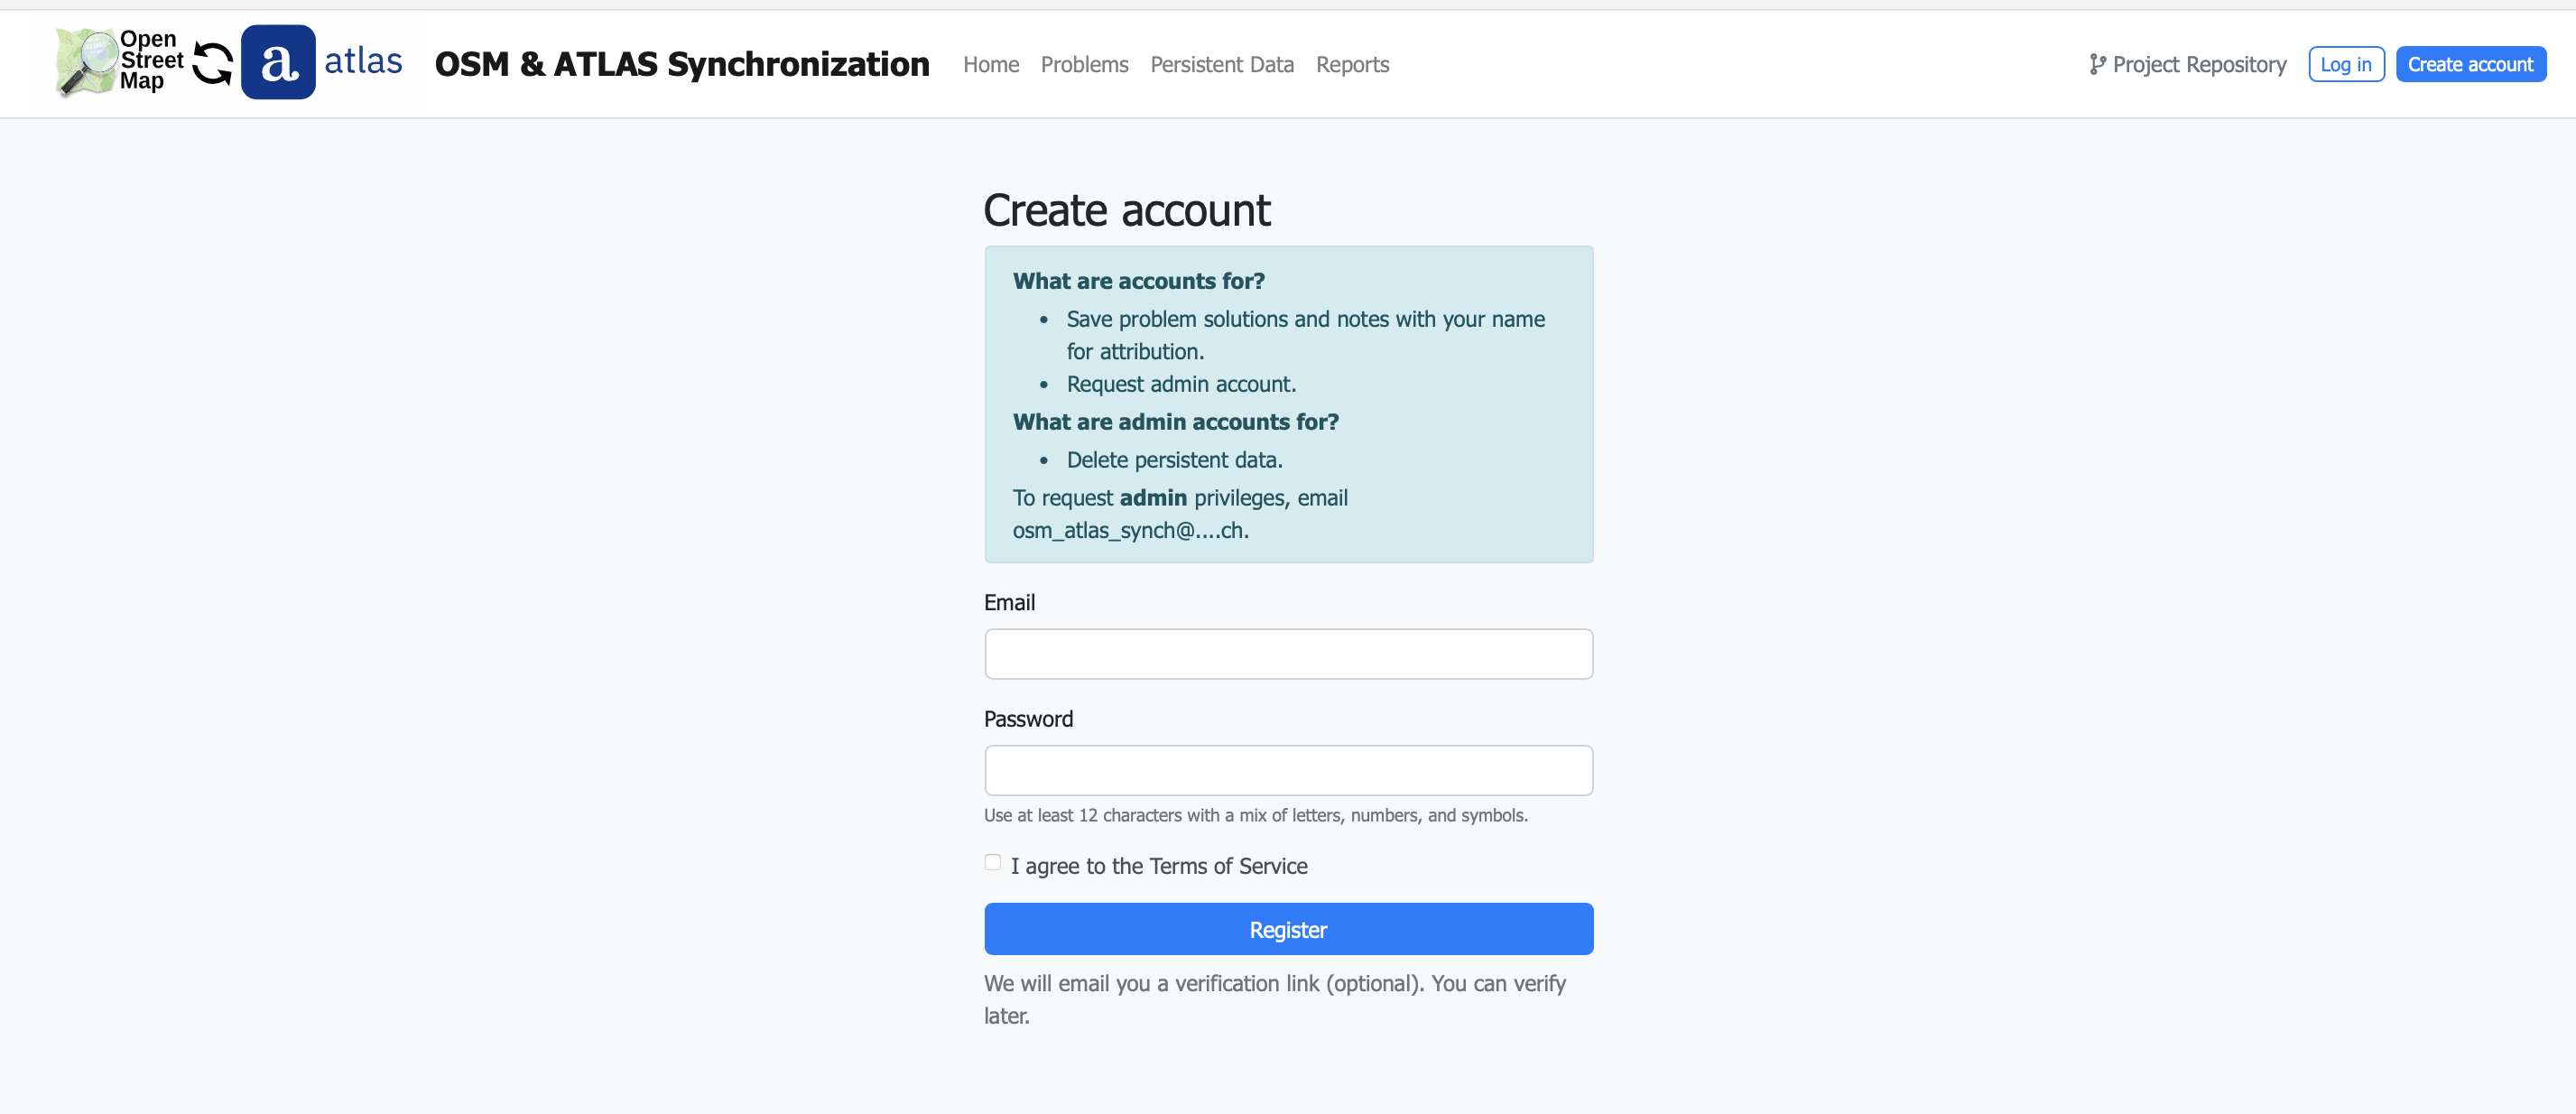
\includegraphics[width=0.85\textwidth]{../figures/chap10/create_account.png}
  \caption{Formulaire d'inscription (email, mot de passe).}
\end{figure}

\begin{figure}[H]
  \centering
  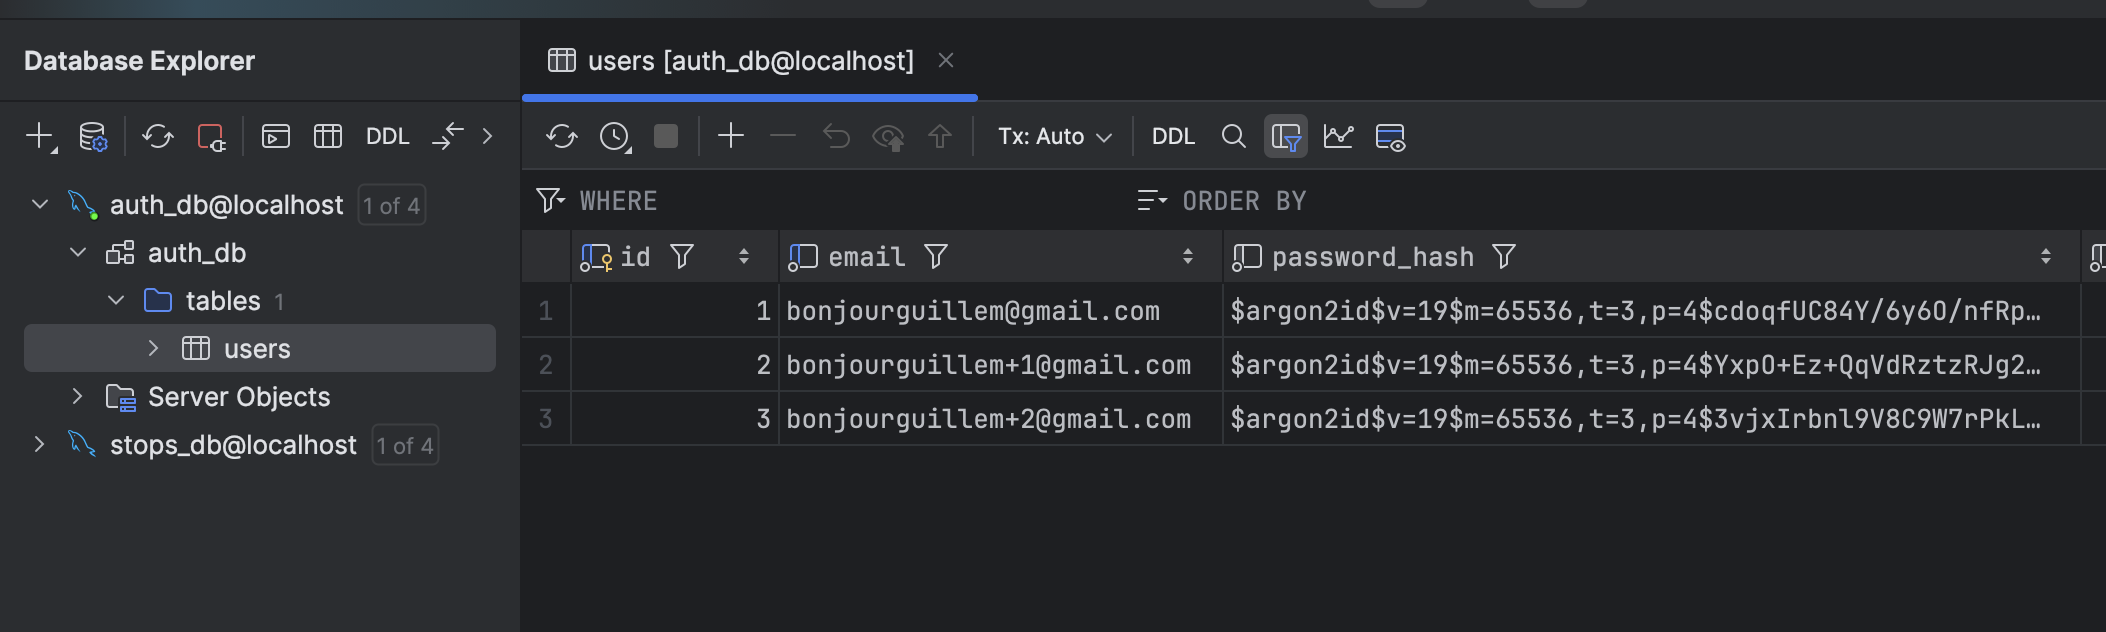
\includegraphics[width=0.85\textwidth]{../figures/chap10/auth_db1.png}
  \caption{\texttt{auth\_db.users}: \texttt{email} et \texttt{password\_hash} après inscription.}
\end{figure}

\paragraph{Vérification d'email}
À l'inscription, un lien de vérification signé (valide 48 h) est envoyé. Lorsqu'un utilisateur non vérifié se connecte avec succès, l'application \textbf{autorise la connexion} et renvoie un nouvel email de vérification accompagné d'un avertissement UI. Des routes dédiées existent pour \textit{vérifier} (\texttt{/auth/verify-email/<token>}) et \textit{renvoyer} (\texttt{/auth/resend-verification}) le lien. Cette vérification peut être rendue obligatoire côté produit si nécessaire.

\begin{figure}[H]
  \centering
  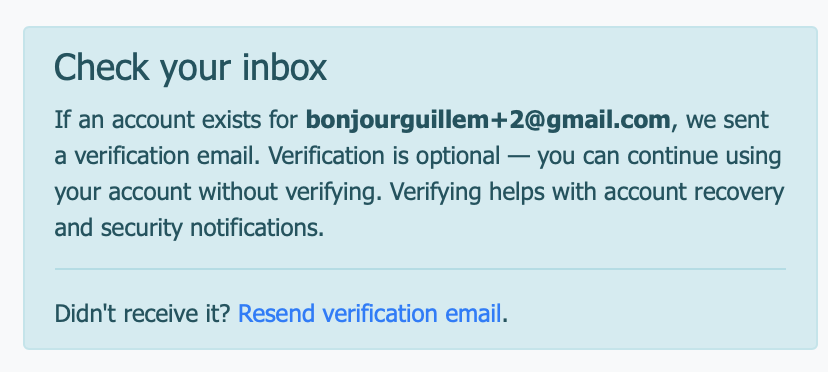
\includegraphics[width=0.85\textwidth]{../figures/chap10/message after clicking email verification.png}
  \caption{Message après avoir demandé une vérification d'email.}
\end{figure}

\begin{codebox}[language=Python]{Jeton de vérification d'email (extrait)}
from itsdangerous import URLSafeTimedSerializer
s = URLSafeTimedSerializer(SECRET_KEY, salt="email-verification")
token = s.dumps({"uid": user_id})
# Plus tard:  uid = int(s.loads(token, max_age=60*60*48)["uid"])  # 48 h
\end{codebox}

\noindent\textbf{Délivrance des emails (Amazon SES)\citeref{ref:aws_ses}.} Les emails de vérification sont rendus côté serveur puis envoyés via Amazon Simple Email Service (SES) grâce au SDK \texttt{boto3}. La fonction \texttt{send\_email(...)} centralise l'envoi dans \texttt{backend/services/email.py} et lit sa configuration via variables d'environnement :
\begin{itemize}
  \item \texttt{AWS\_REGION} (p.~ex. \texttt{eu-west-1})
  \item \texttt{SES\_FROM\_EMAIL} (identité SES vérifiée)
  \item \texttt{SES\_CONFIGURATION\_SET} (optionnel)
\end{itemize}
Le flux d'envoi est déclenché depuis \texttt{backend/blueprints/auth.py} : l'application génère le lien signé, rend les gabarits d'email (HTML et texte) dans \texttt{templates/emails/}, puis appelle \texttt{send\_email(...)}. Les erreurs d'envoi sont journalisées mais n'interrompent pas le parcours utilisateur, afin d'éviter toute fuite d'information et de préserver l'ergonomie.

\begin{figure}[H]
  \centering
  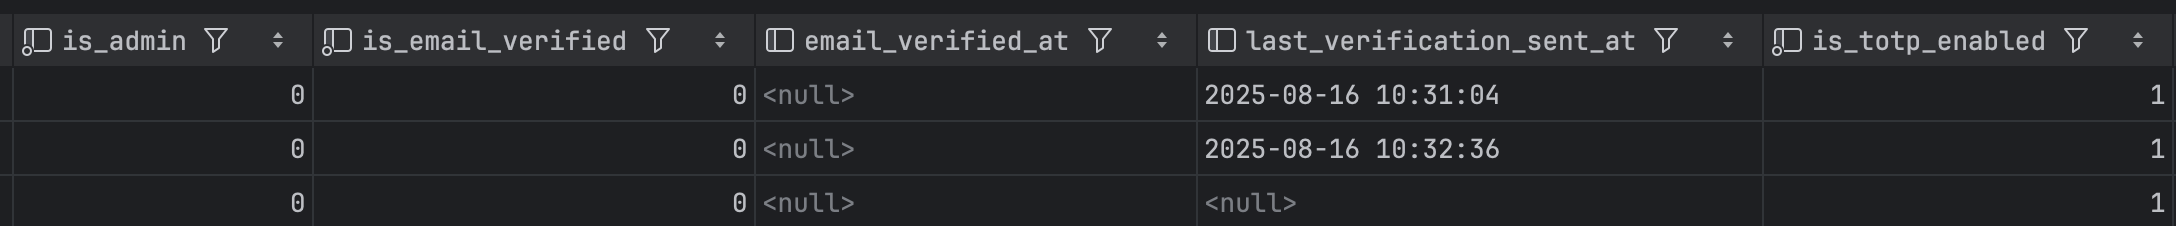
\includegraphics[width=0.85\textwidth]{../figures/chap10/auth_db2.png}
  \caption{\texttt{auth\_db.users}: \texttt{is\_admin}, \texttt{is\_email\_verified}, \texttt{last\_verification\_sent\_at}, \texttt{is\_totp\_enabled}.}
\end{figure}

\paragraph{Connexion}
L'utilisateur s'authentifie sur la page de connexion ; en cas de succès, l'application met à jour l'historique de connexion et applique le verrouillage en cas d'échecs répétés.

\begin{figure}[H]
  \centering
  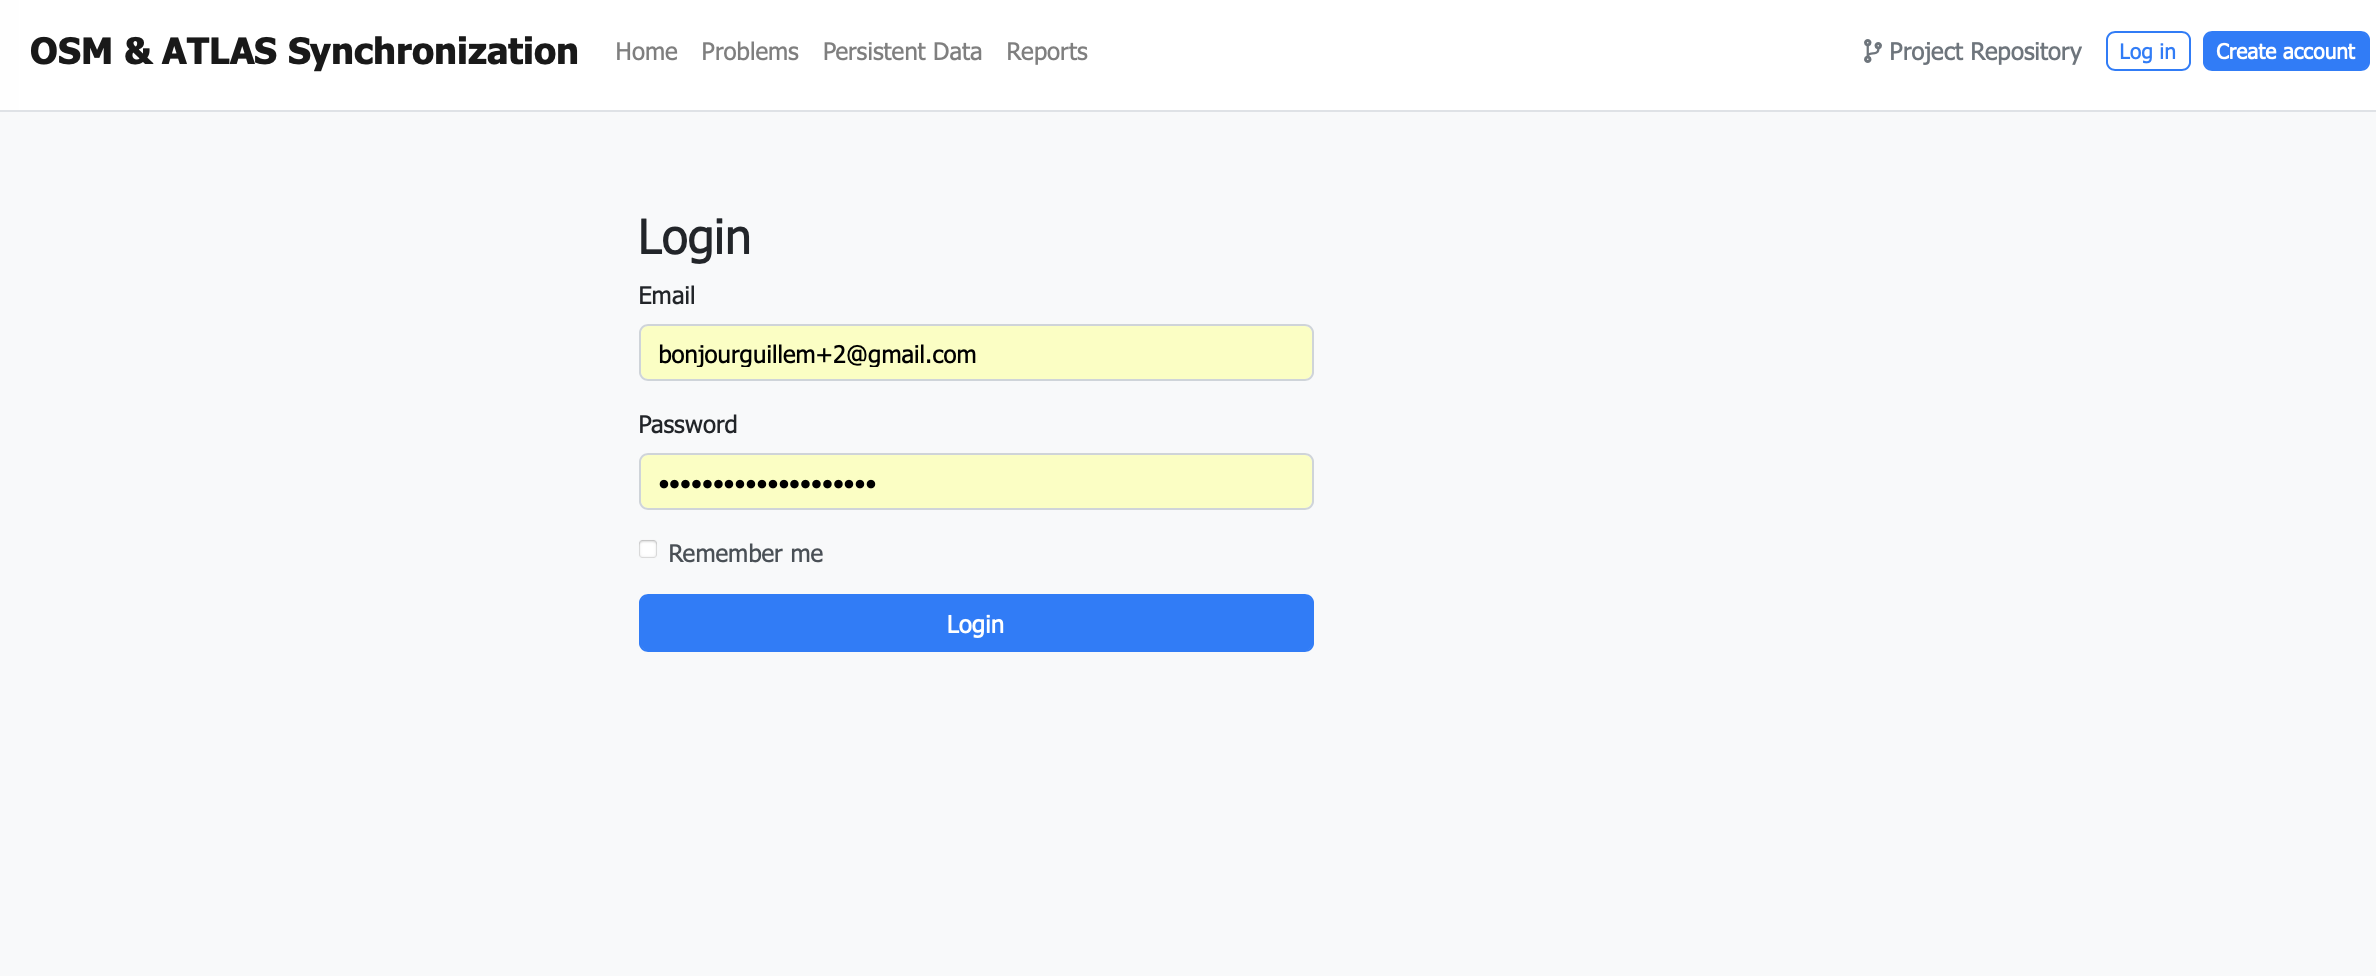
\includegraphics[width=0.85\textwidth]{../figures/chap10/login_page.png}
  \caption{Page de connexion. Les limites de débit et le CAPTCHA (Turnstile) freinent les robots (voir Chap.~\ref{chap:auth}).}
\end{figure}

\begin{figure}[H]
  \centering
  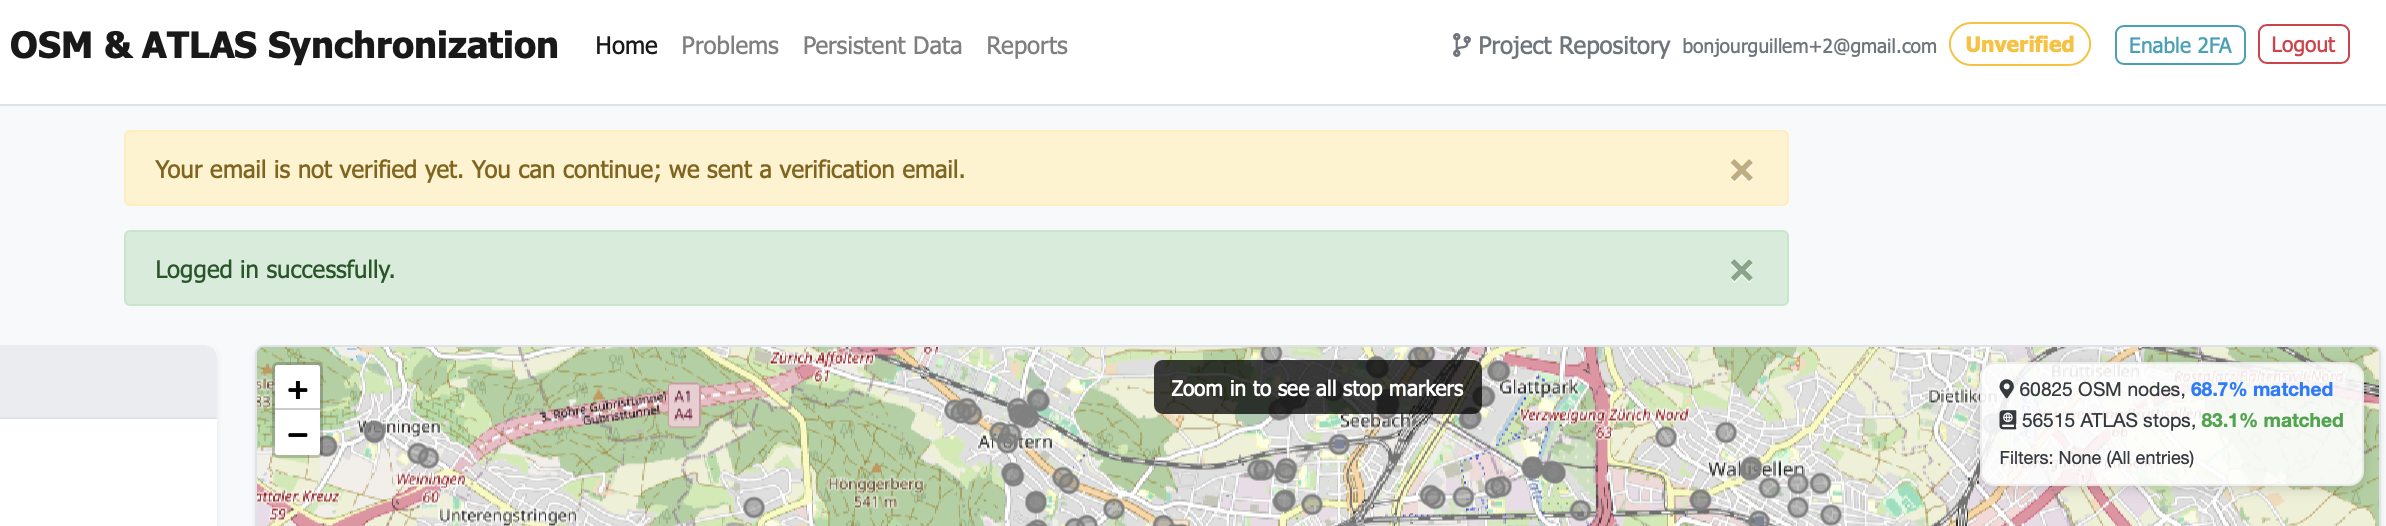
\includegraphics[width=0.85\textwidth]{../figures/chap10/login_succesful.png}
  \caption{Connexion réussie : alertes UI sur l'email non vérifié et la 2FA non activée.}
\end{figure}

\begin{figure}[H]
  \centering
  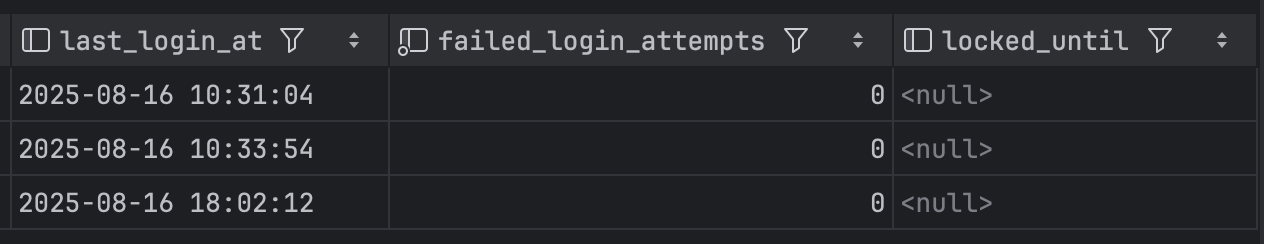
\includegraphics[width=0.85\textwidth]{../figures/chap10/auth_db4.png}
  \caption{\texttt{auth\_db.users}: \texttt{last\_login\_at}, \texttt{failed\_login\_attempts}, \texttt{locked\_until}.}
\end{figure}

\paragraph{2FA}
Lorsqu'un utilisateur active la 2FA, le serveur génère un secret Base32 aléatoire et affiche un QR code contenant une URI \textit{otpauth} standard. \textbf{Ce secret est chiffré au repos} (\texttt{cryptography.Fernet}) avec une clé d'application fournie par variable d'environnement, puis stocké dans \texttt{auth\_db.users.totp\_secret}. L'utilisateur vérifie le premier code à 6 chiffres pour activer la 2FA. Le serveur génère 10 codes de secours à usage unique et n'en stocke que les versions hachées avec Argon2. À la connexion, si la 2FA est active, l'utilisateur doit fournir un TOTP valide ou un code de secours non utilisé.

\begin{figure}[H]
  \centering
  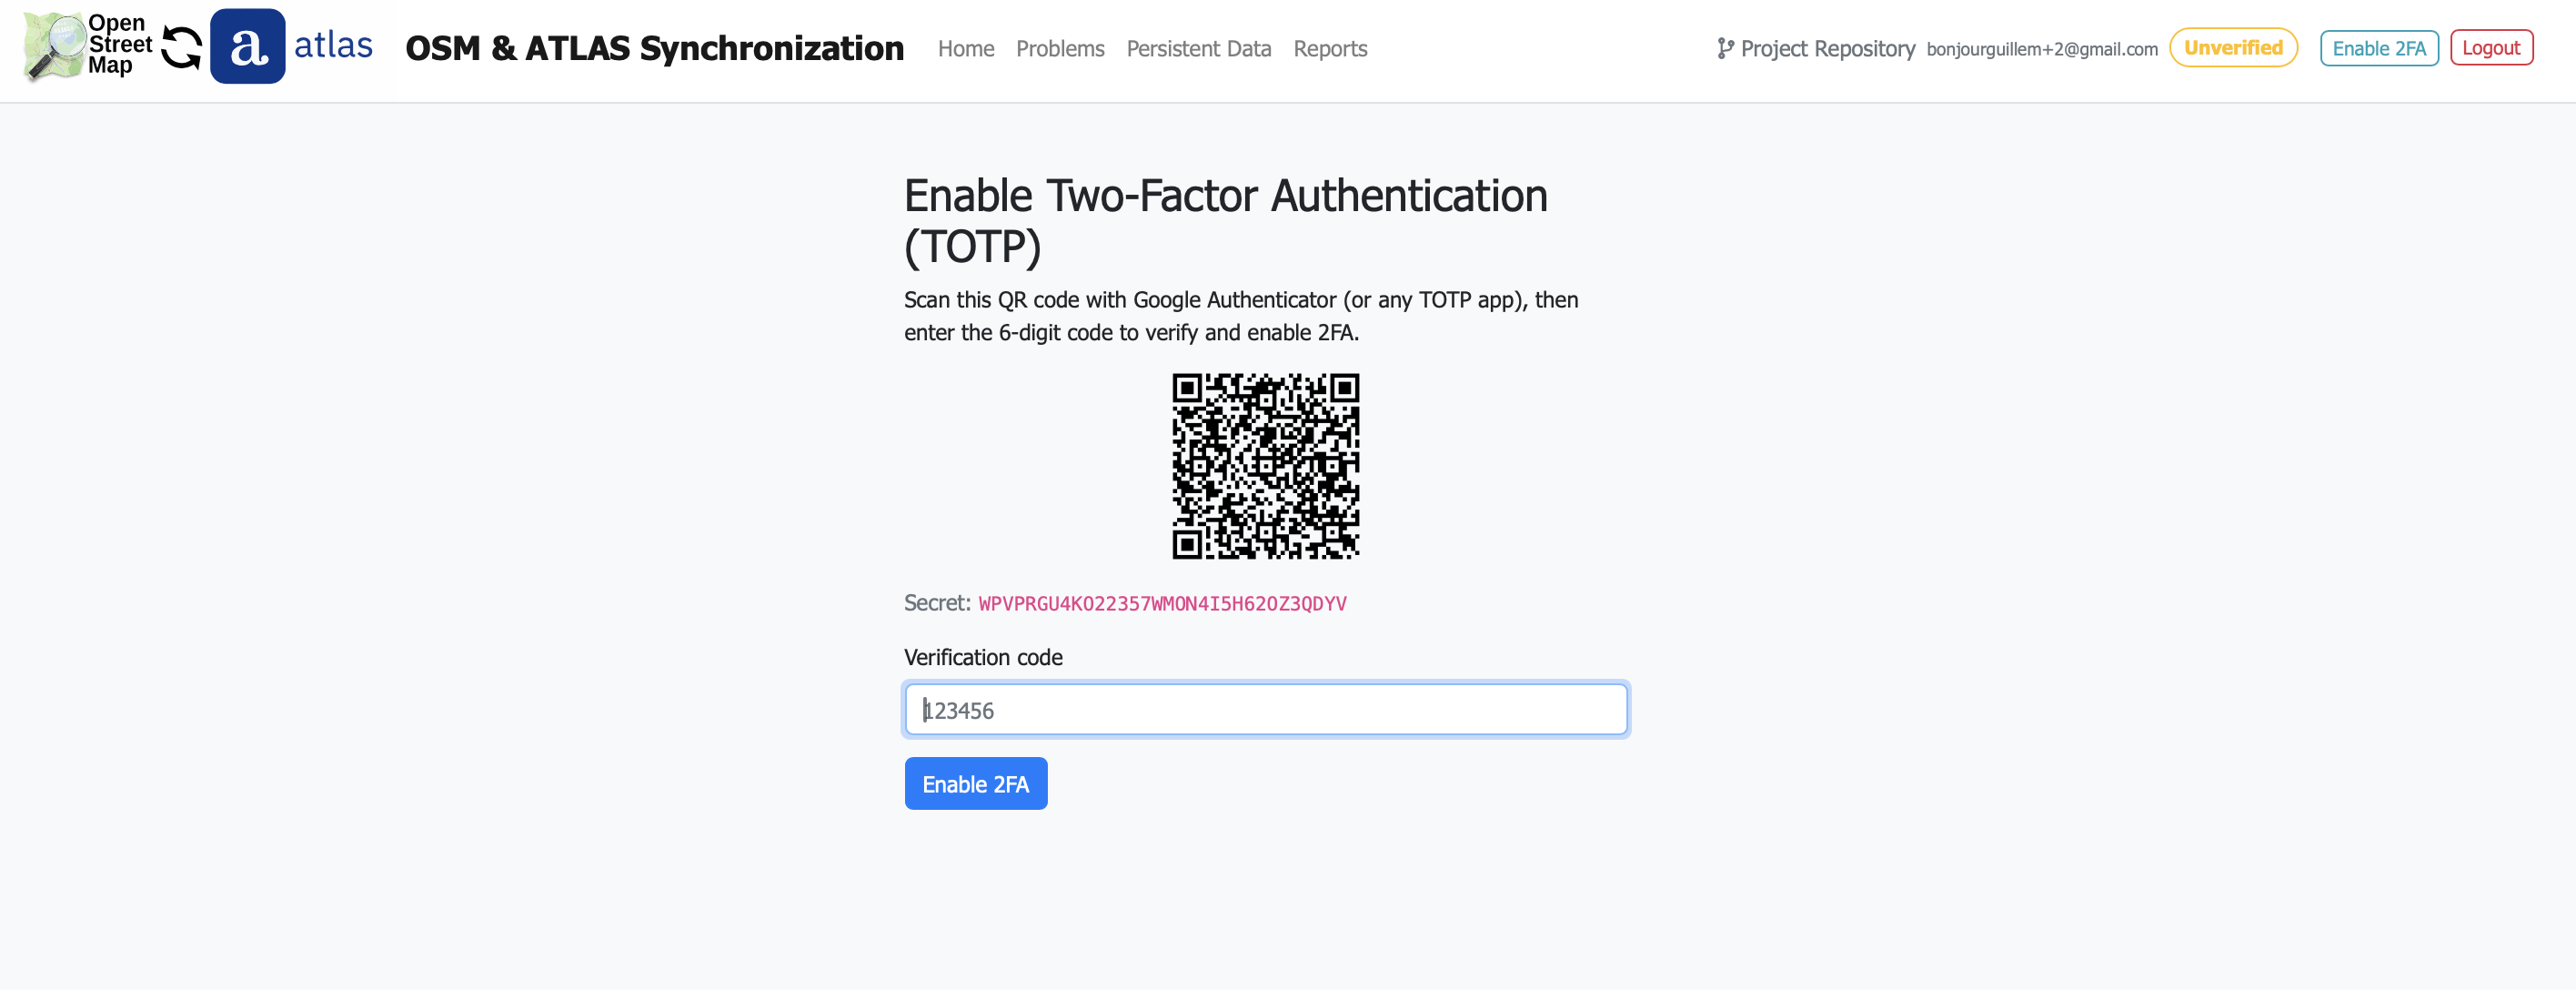
\includegraphics[width=0.85\textwidth]{../figures/chap10/enable_up2fa.png}
  \caption{Activation 2FA avec QR \textit{otpauth://} et secret Base32. QR et secret encodent la même information.}
\end{figure}

\begin{codebox}[language=Python]{Validation TOTP (connexion avec 2FA)}
import pyotp
secret = user.get_totp_secret()  # déchiffre à la volée si chiffré
is_valid = pyotp.TOTP(secret).verify(code, valid_window=1)
\end{codebox}

\begin{figure}[H]
  \centering
  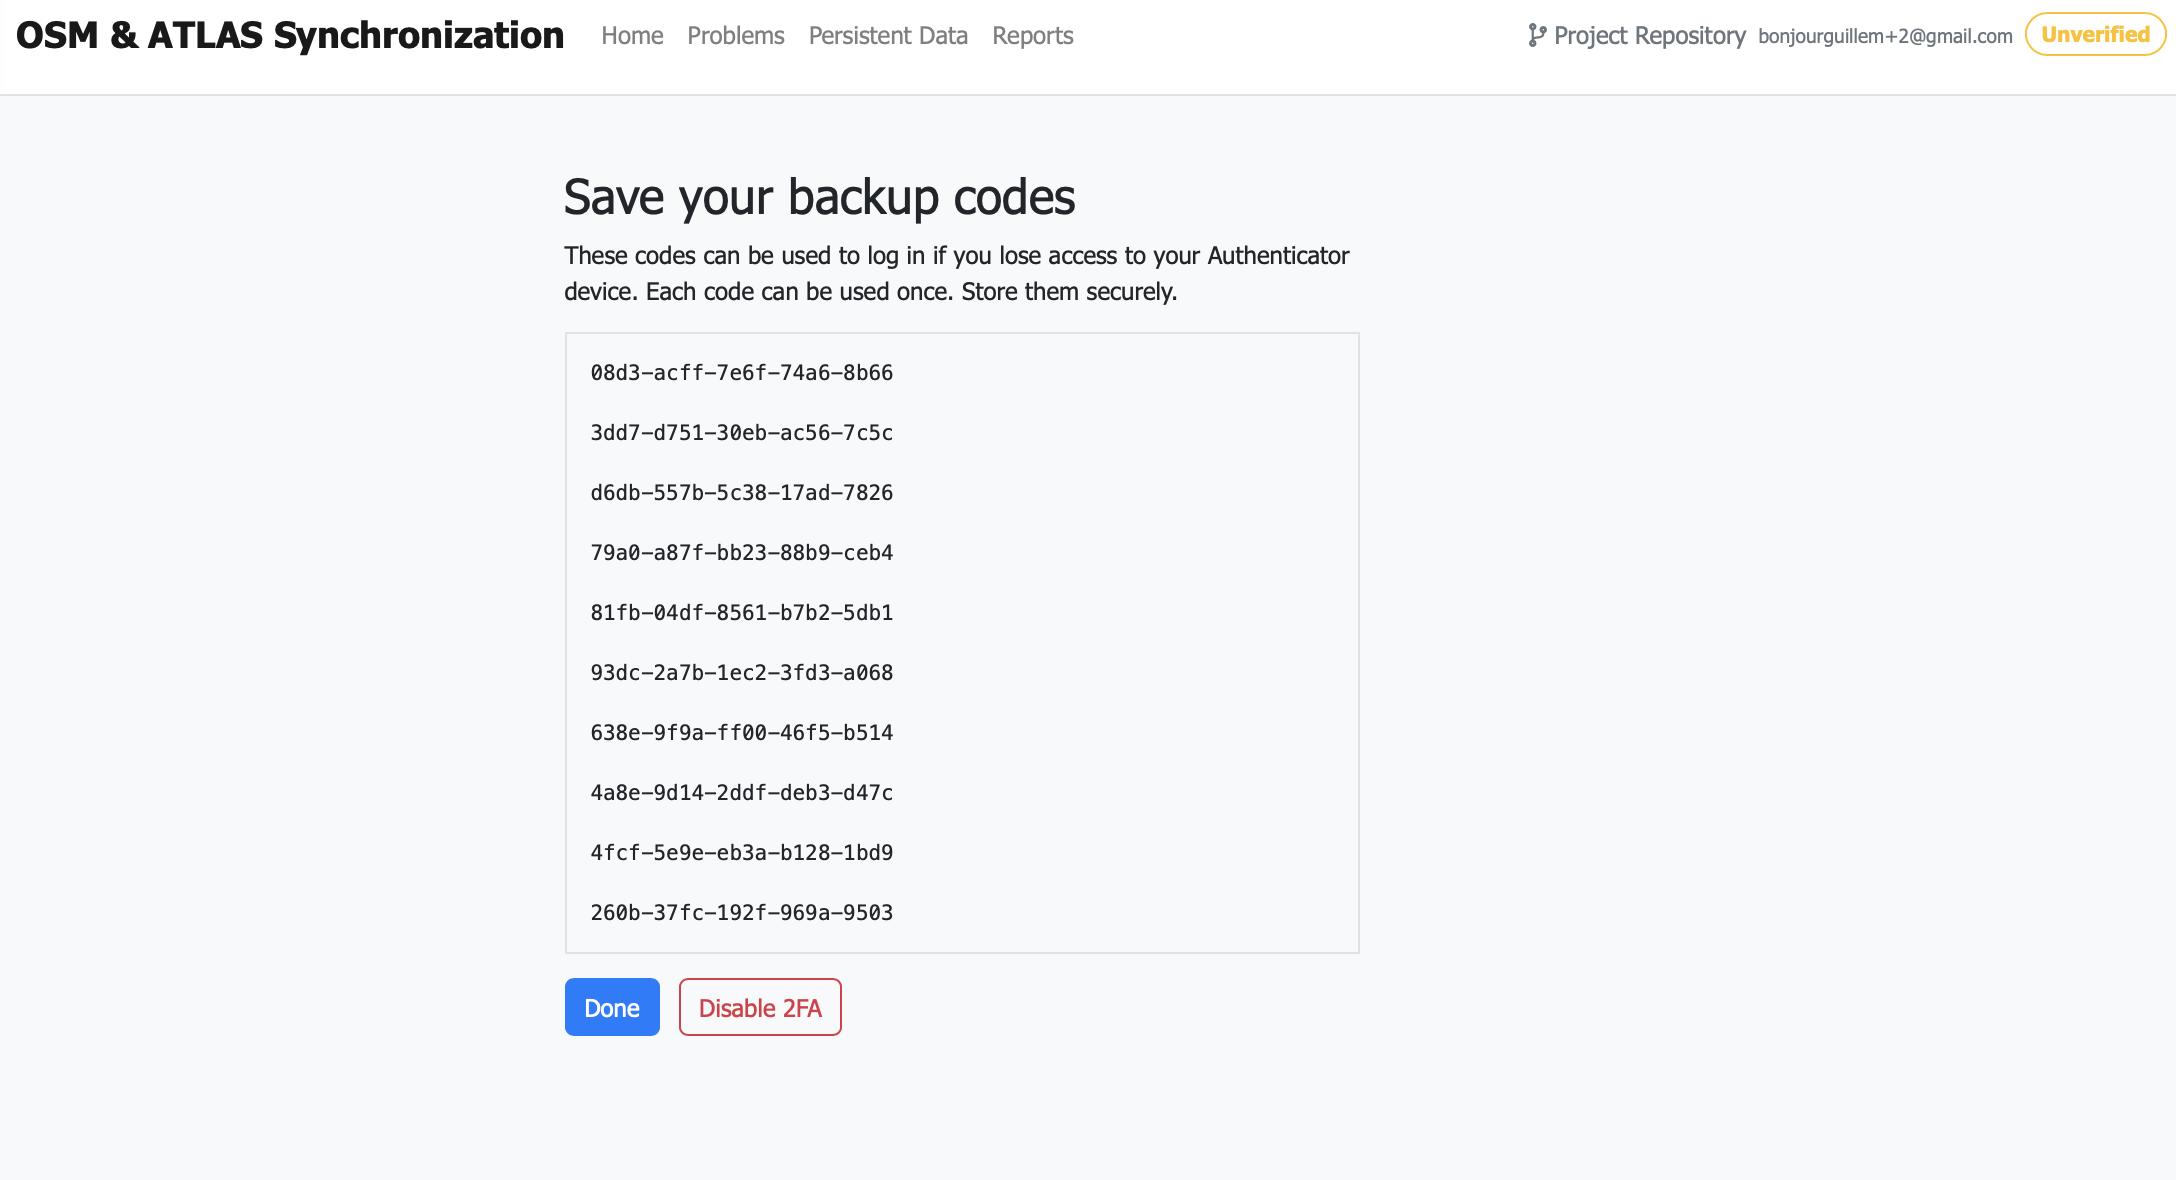
\includegraphics[width=0.85\textwidth]{../figures/chap10/backupcodes.png}
  \caption{Codes de secours: affichés une seule fois à l'activation. Stockage côté serveur: hachés Argon2 dans un JSON.}
\end{figure}

\begin{figure}[H]
  \centering
  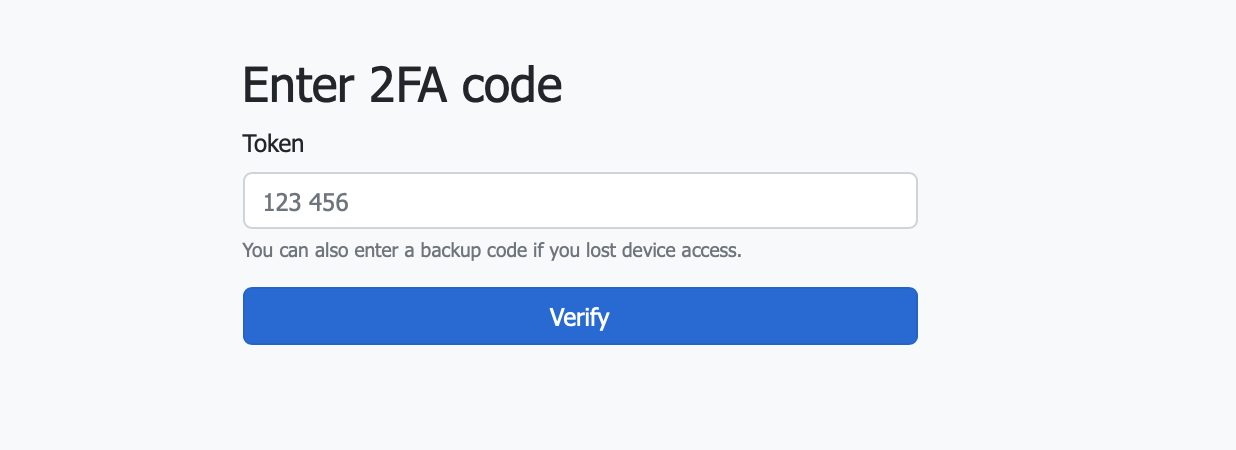
\includegraphics[width=0.85\textwidth]{../figures/chap10/enter2FA.png}
  \caption{Étape de connexion avec saisie du code 2FA (ou d'un code de secours).}
\end{figure}

\begin{figure}[H]
  \centering
  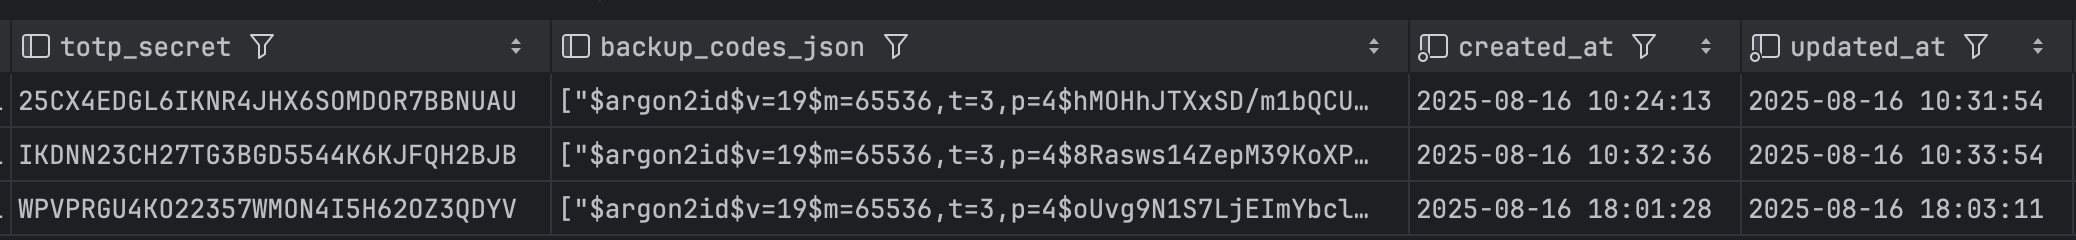
\includegraphics[width=0.85\textwidth]{../figures/chap10/auth_db3.png}
  \caption{\texttt{auth\_db.users}: \texttt{totp\_secret} (chiffré), \texttt{backup\_codes\_json} (haché), \texttt{created\_at}, \texttt{updated\_at}.}
\end{figure}

\section{Sécurité opérationnelle (en pratique)}
\noindent Cette section résume les mesures concrètes d'exploitation sécurisée et l'intention derrière chacune.

\begin{itemize}
  \item \textbf{Secrets et configuration} : Les clés d'application (\texttt{SECRET\_KEY}), URL de base (\texttt{AUTH\_DATABASE\_URI}) et HTTPS sont fournis par variables d'environnement (Docker Compose). Ils ne sont jamais versionnés.
  \item \textbf{Mots de passe et codes} : Rien n'est stocké en clair. Les mots de passe sont hachés (Argon2id) ; les codes de secours sont également hachés.
  \item \textbf{Moindre privilège} : \texttt{auth\_db} utilise des comptes dédiés avec des droits minimaux ; chaque service n'accède qu'au strict nécessaire.
  \item \textbf{Protection contre les attaques} : Limitation de débit, verrouillage progressif et CAPTCHA atténuent la force brute et le bourrage d'identifiants.
  \item \textbf{En-têtes et CSP} : Talisman applique les en-têtes de sécurité et une politique CSP. Cette CSP peut être durcie en réduisant l'usage de CDN.
  \item \textbf{Traçabilité} : Les événements d'authentification sont consignés dans \texttt{auth\_events} et envoyés en logs JSON pour la supervision.
\end{itemize}




